\section{Projeto de controlador por \textit{state feedback}}

\subsection{Método utilizando fórmula de Ackermann}

O desempenho escolhido para o sistema foi de $e.r = 0$ para $r(t) = 1$, $T_s_2\% \leq 4s$ e $PO\% \leq 5\%$.
Inicialmente, se obteve a equação no tempo para que se possa conseguir as matrizes de estado da planta, e assim se fazer os devidos cálculos de realimentação de estados. Dessa forma, temos:
\begin{center}
    $G_p(s) = \frac{Y(s)}{X(s)} = \frac{2}{s(s+0,5)}$ \vspace{7pt}\\
    $s^2Y(s) + 0,5sY(s) = 2U(s)$ \vspace{5pt}\\
    $\Ddot{y}(t) + 0,5\Dot{y} = 2u$
\end{center}
Com isso, fazemos:
\begin{center}
    $\left\{\begin{array}{ll}x_1=y\\x_2=\Dot{y}\end{array}\right$
\end{center}
E teremos:
\begin{center}
     $\left\{\begin{array}{ll}\Dot{x_1}=x_2\\x_2=2u-0,5x_1\end{array}\right$
\end{center}
Nos dando, por fim, as matrizes de estado da planta:
\begin{center}
    $\left\{\begin{array}{ll}\Dot{x}$ = $\left[  \begin{array}{cc} 0 & 1\\ -0,5 & 0\\ \end{array} \right] \left[  \begin{array}{c} x_1\\ x_2\\ \end{array} \right]  + \left[  \begin{array}{c} 0\\ 2\\ \end{array} \right] u(t) \vspace{5pt}\\ y = \left[  \begin{array}{cc} 1 & 0 \end{array} \right] \left[  \begin{array}{c} x_1\\ x_2\\ \end{array} \right]\end{array}\right$
\end{center}

Agora, com as matrizes do espaço de estado tidas, vamos encontrar o polinômio característico do sistema com o desempenho desejado. Para o potencial de \textit{overshoot} de $5\%$, por tabela temos um $\xi = 0,7$, além de um ângulo $\theta = 45\degree$. Para um tempo de estabilização de 4 segundos, pela equação, teremos $-\xi \omega_n = -1$. Com isso, $\omega_n = 1,43$. Temos então a equação:
\begin{center}
    $a^* = s^2 + 2s + 2,041$
\end{center}

Antes de encontrarmos o vetor K para a realimentação de estado, precisamos saber qual sua matriz de controlabilidade e, por meio dela, se o sistema é controlável. Com isso, temos:
\begin{center}
    $W_c = \left[  \begin{array}{cc} B & AB \end{array} \right]$
    $W_c = \left[  \begin{array}{cc} 0 & 2\\ 2 & 0 \end{array} \right]$
\end{center}

Com a matriz, basta retirar o determinante. Se o mesmo for diferente de 0, o sistema é controlável.
\begin{center}
    $det(W_c) = -(2*2) = -4 \neq 0$
\end{center}

Com o polinômio característico e a matriz de controlabilidade, podemos utilizar a fórmula de Ackermann. A fórmula nos dá uma forma de encontrar o vetor de ganhos K utilizando esses dois parâmetros encontrados:
\begin{center}
    $K = \left[  \begin{array}{cc} 0 & 1 \end{array} \right] W_c^{-1} \Phi$
\end{center}
Onde $\Phi$ é o polinômio característico com a substituição de s pela matriz A:
\begin{center}
    $\Phi = A^2 + 2A + 2,041I$ \vspace{5pt}\\
    $\Phi = \left[  \begin{array}{cc} 1,541 & 2\\ -1 & 1,541 \end{array} \right]$
\end{center}
Logo, temos que K será:
\begin{center}
    $K = \left[  \begin{array}{cc} 0 & 1 \end{array} \right] \left[  \begin{array}{cc} 0 & 2\\ 2 & 0 \end{array} \right]^{-1} \left[  \begin{array}{cc} 1,541 & 2\\ -1 & 1,541 \end{array} \right]$ \vspace{7pt}\\
    $K = \left[  \begin{array}{cc} 0,7705 & 1 \end{array} \right]$ \vspace{5pt}\\
    \boxed{K_1 = 0,7705} e \boxed{K_2 = 1}
\end{center}

\subsection{Simulações no Scilab}
Com os cálculos feitos, foi utilizada a ferramenta \textbf{XCOS} do software \textbf{Scilab} para construir o diagrama de blocos e parametrizá-los. 
Para facilitar a formulação do circuito, se considerou o $K_1 = 1$ e não igual a 0,7705, como visto anteriormente. Com isso, houve uma mudança pouco perceptível, e o sistema continuou garantindo os requisitos. Nas figuras ~\ref{xcos:state:a} e ~\ref{xcos:state:b}, é possível ver que a mudança pouco modificou o resultado final que se deseja obter.

\begin{figure}[H]
\begin{center}
    \subfigure[Diagrama de blocos]{             
        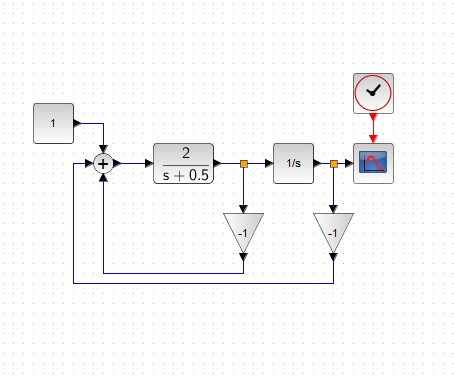
\includegraphics[width=6cm]{images/state/diag_state.jpg}  
        \label{xcos:state:a}
    }
    \subfigure[Simulação temporal]{                                              
        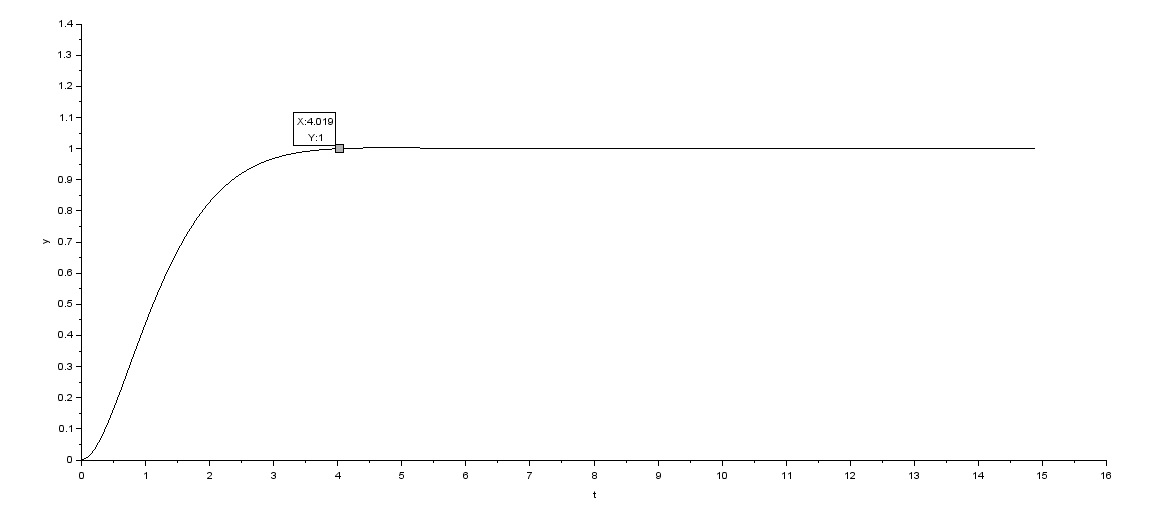
\includegraphics[width=9.5cm]{images/state/time_state.jpg}
        \label{xcos:state:b}
    }                
\end{center}
\caption{Simulação com o sistema planta+controlador realimentação de estado no XCOS.}
\label{xcos:state} 
\end{figure}

Desta forma, por meio das simulações, é possível perceber que a estabilidade e o desempenho desejados foram satisfeito, mesmo que com alguns arredondamentos considerados bruscos. Obtemos um tempo de estabilização em torno dos 4 segundos, além de termos um \textit{overshoot} em torno de 3\% no sistema.

%\pagebreak